\documentclass[letter]{article}
\renewcommand{\baselinestretch}{1.25}

\usepackage[margin=1in]{geometry}
\usepackage{physics}
\usepackage{amsmath, mathtools}
\numberwithin{equation}{section}
\usepackage{amssymb}
\usepackage{graphicx}
\usepackage{hyperref}
\usepackage{empheq}

% MATLAB Formating Code
\usepackage[numbered,framed]{matlab-prettifier}
\lstset{style=Matlab-editor,columns=fullflexible}
\renewcommand{\lstlistingname}{Script}
\newcommand{\scriptname}{\lstlistingname}

\allowdisplaybreaks

%opening
\title{MECH 6323 - HW 1}
\author{Jonas Wagner}
\date{2022, January 24}

\begin{document}	

\maketitle

% \tableofcontents

%----------------------------------------------------------------------------
% \newpage
\section{Problem 1}









\newpage
\section{Problem 3}
\textbf{Problem:}
For each of the bode plots:
\begin{enumerate}
	\item Determine the breakpoints and the transfer function.
	\item Determine the gain cross-over frequency $\omega_c$ and the phase cross-over frequency $\omega_{180}$.
\end{enumerate}

\subsection{Bode Plot 1:}
\begin{figure}[h]
	\centering
	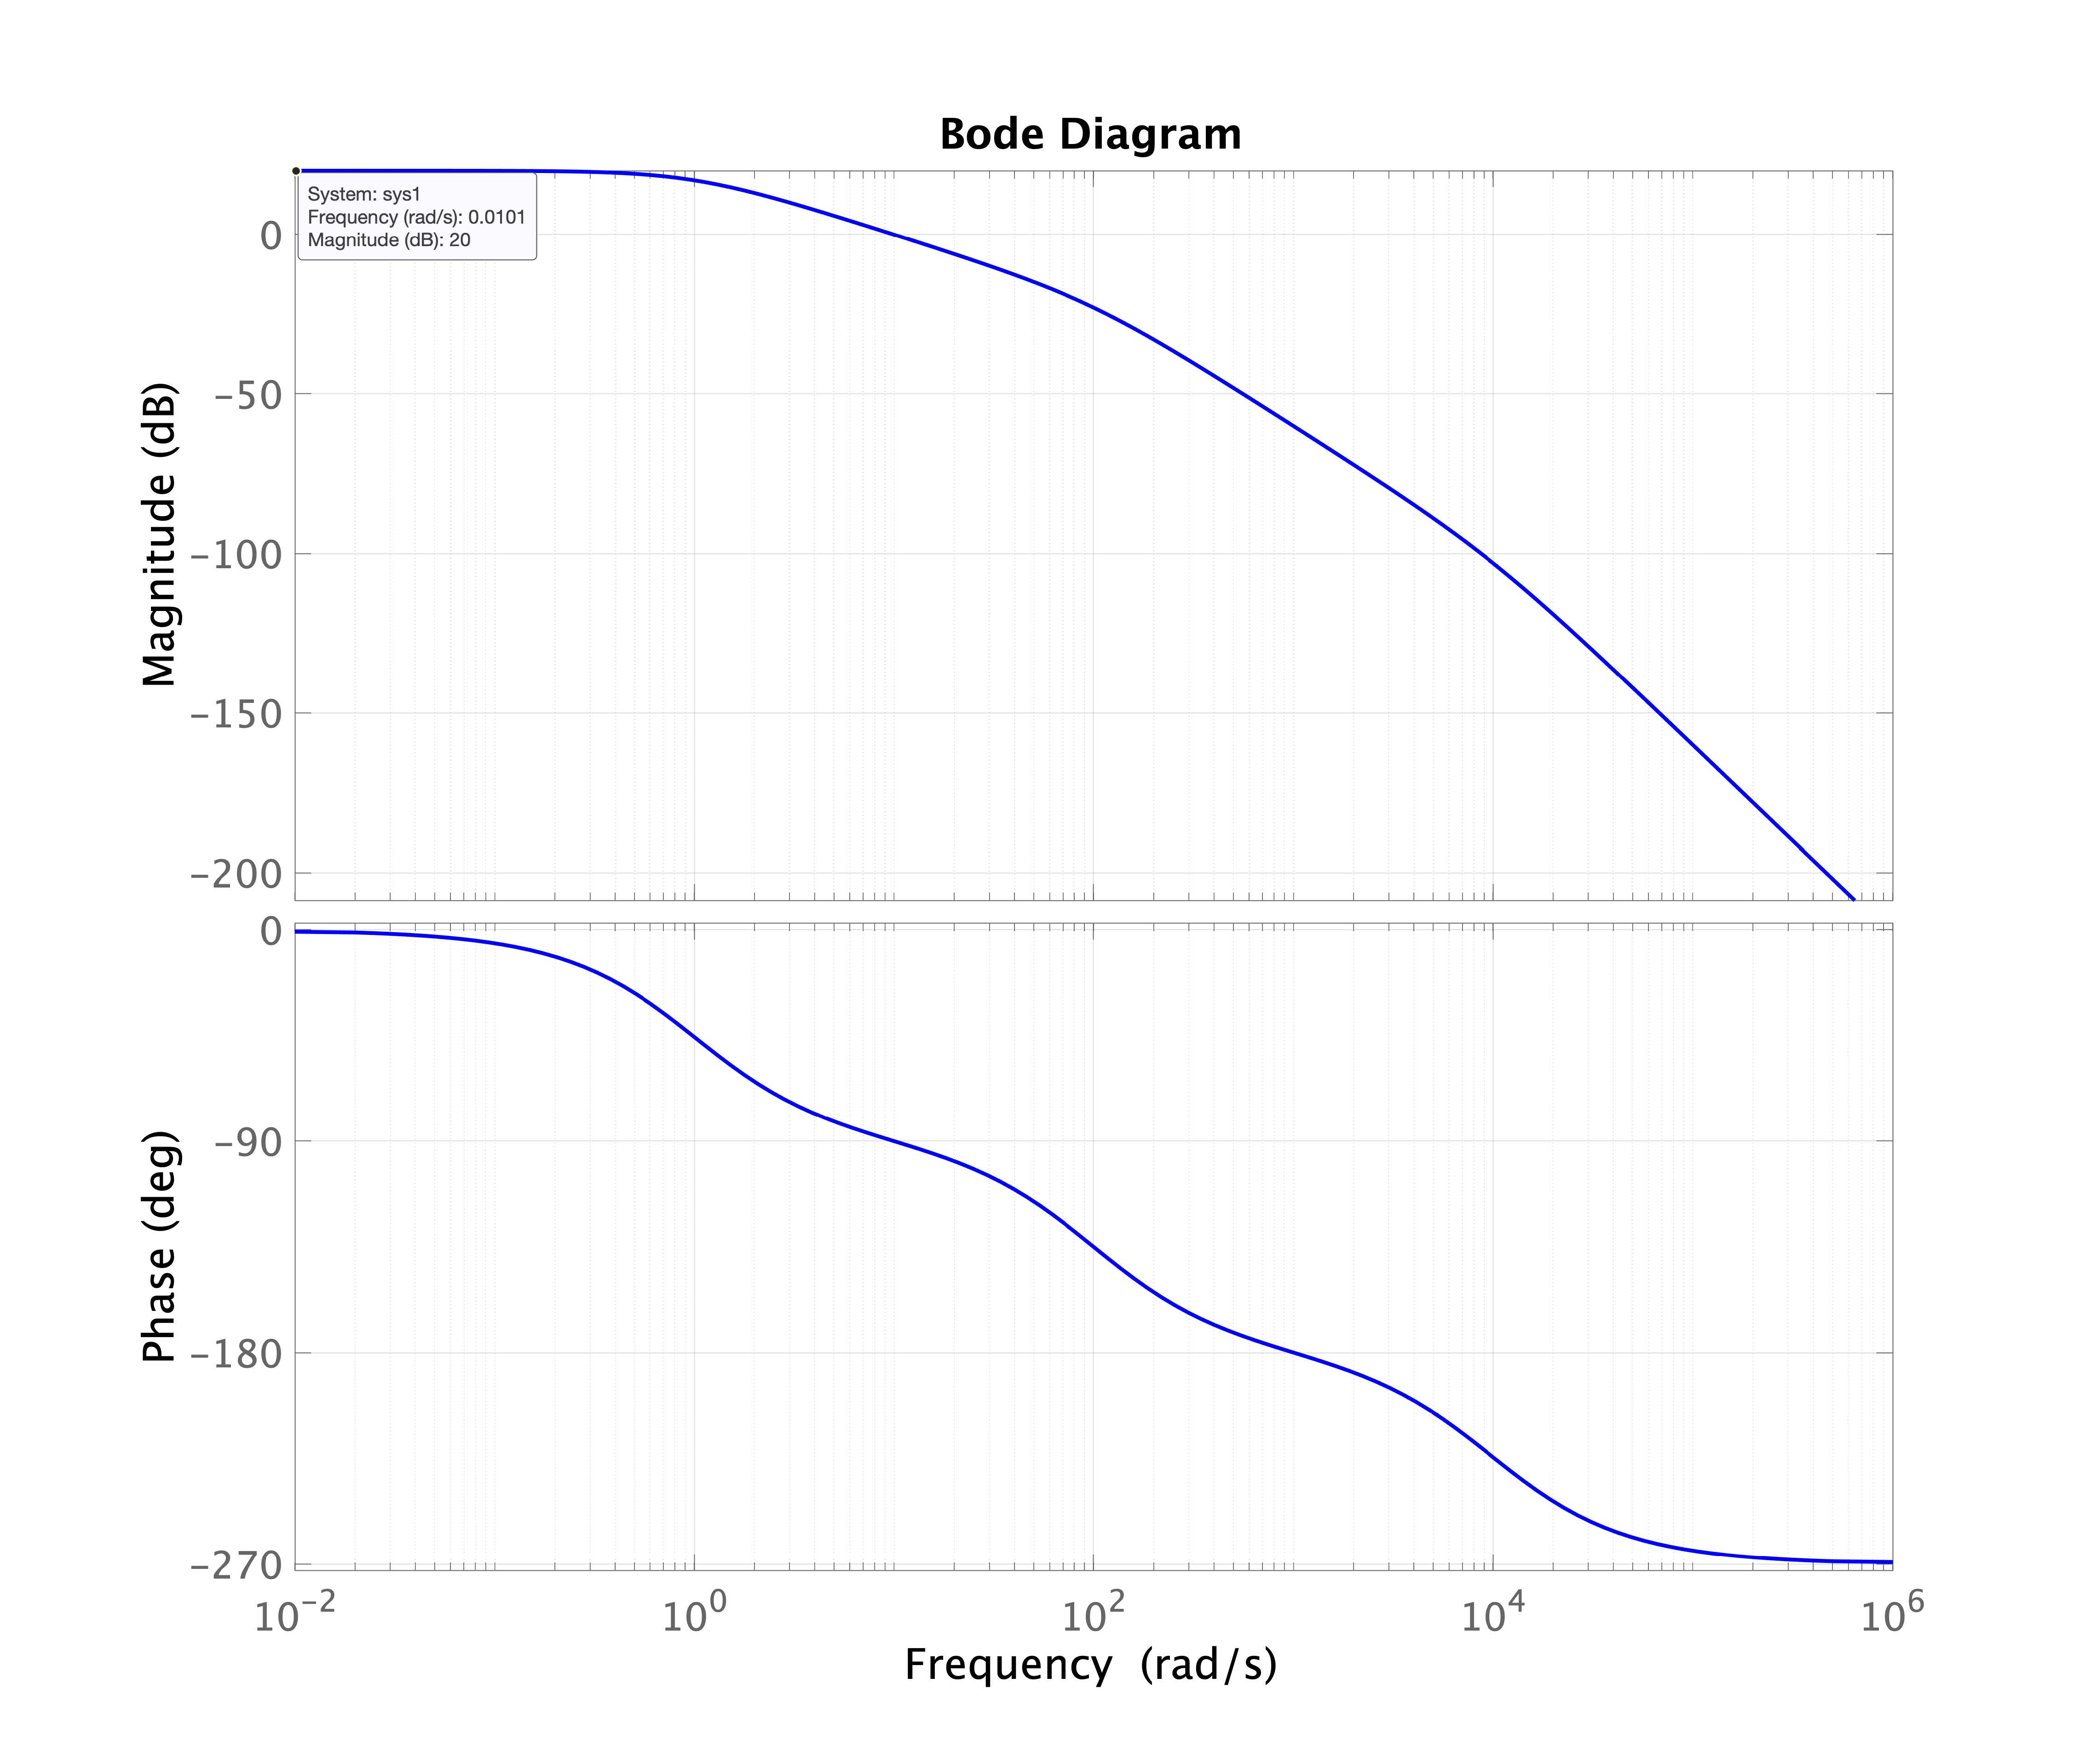
\includegraphics[width=0.5\textwidth]{figs/pblm3a.jpg}
\end{figure}

\subsubsection{Gain, Poles, and Zeros:}
\begin{enumerate}
	\item \textbf{Gain:}  $20$ db = 10
	\item \textbf{Poles:}
	\begin{enumerate}
		\item $10^{0} = 1$ rad/s
		\item $10^{2} = 100$ rad/s
		\item $10^{4} = 10,000$ rad/s
	\end{enumerate}
	\item Zeros: (NA)
\end{enumerate}

\textbf{Transfer Function:}\[
	H(s) = \cfrac{10}{
		\qty(1 + \frac{s}{1}) \qty(1 + \frac{s}{100}) \qty(1 + \frac{s}{10000})
		}
\]

\subsubsection{Cross-over Frequency:}
\begin{enumerate}
	\item $\omega_c = 10^{1} = 10$ rad/s
	\item $\omega_{180} = 10^{3} = 100$ rad/s
\end{enumerate}



\newpage
\subsection{Bode Plot 2:}
\begin{figure}[h]
	\centering
	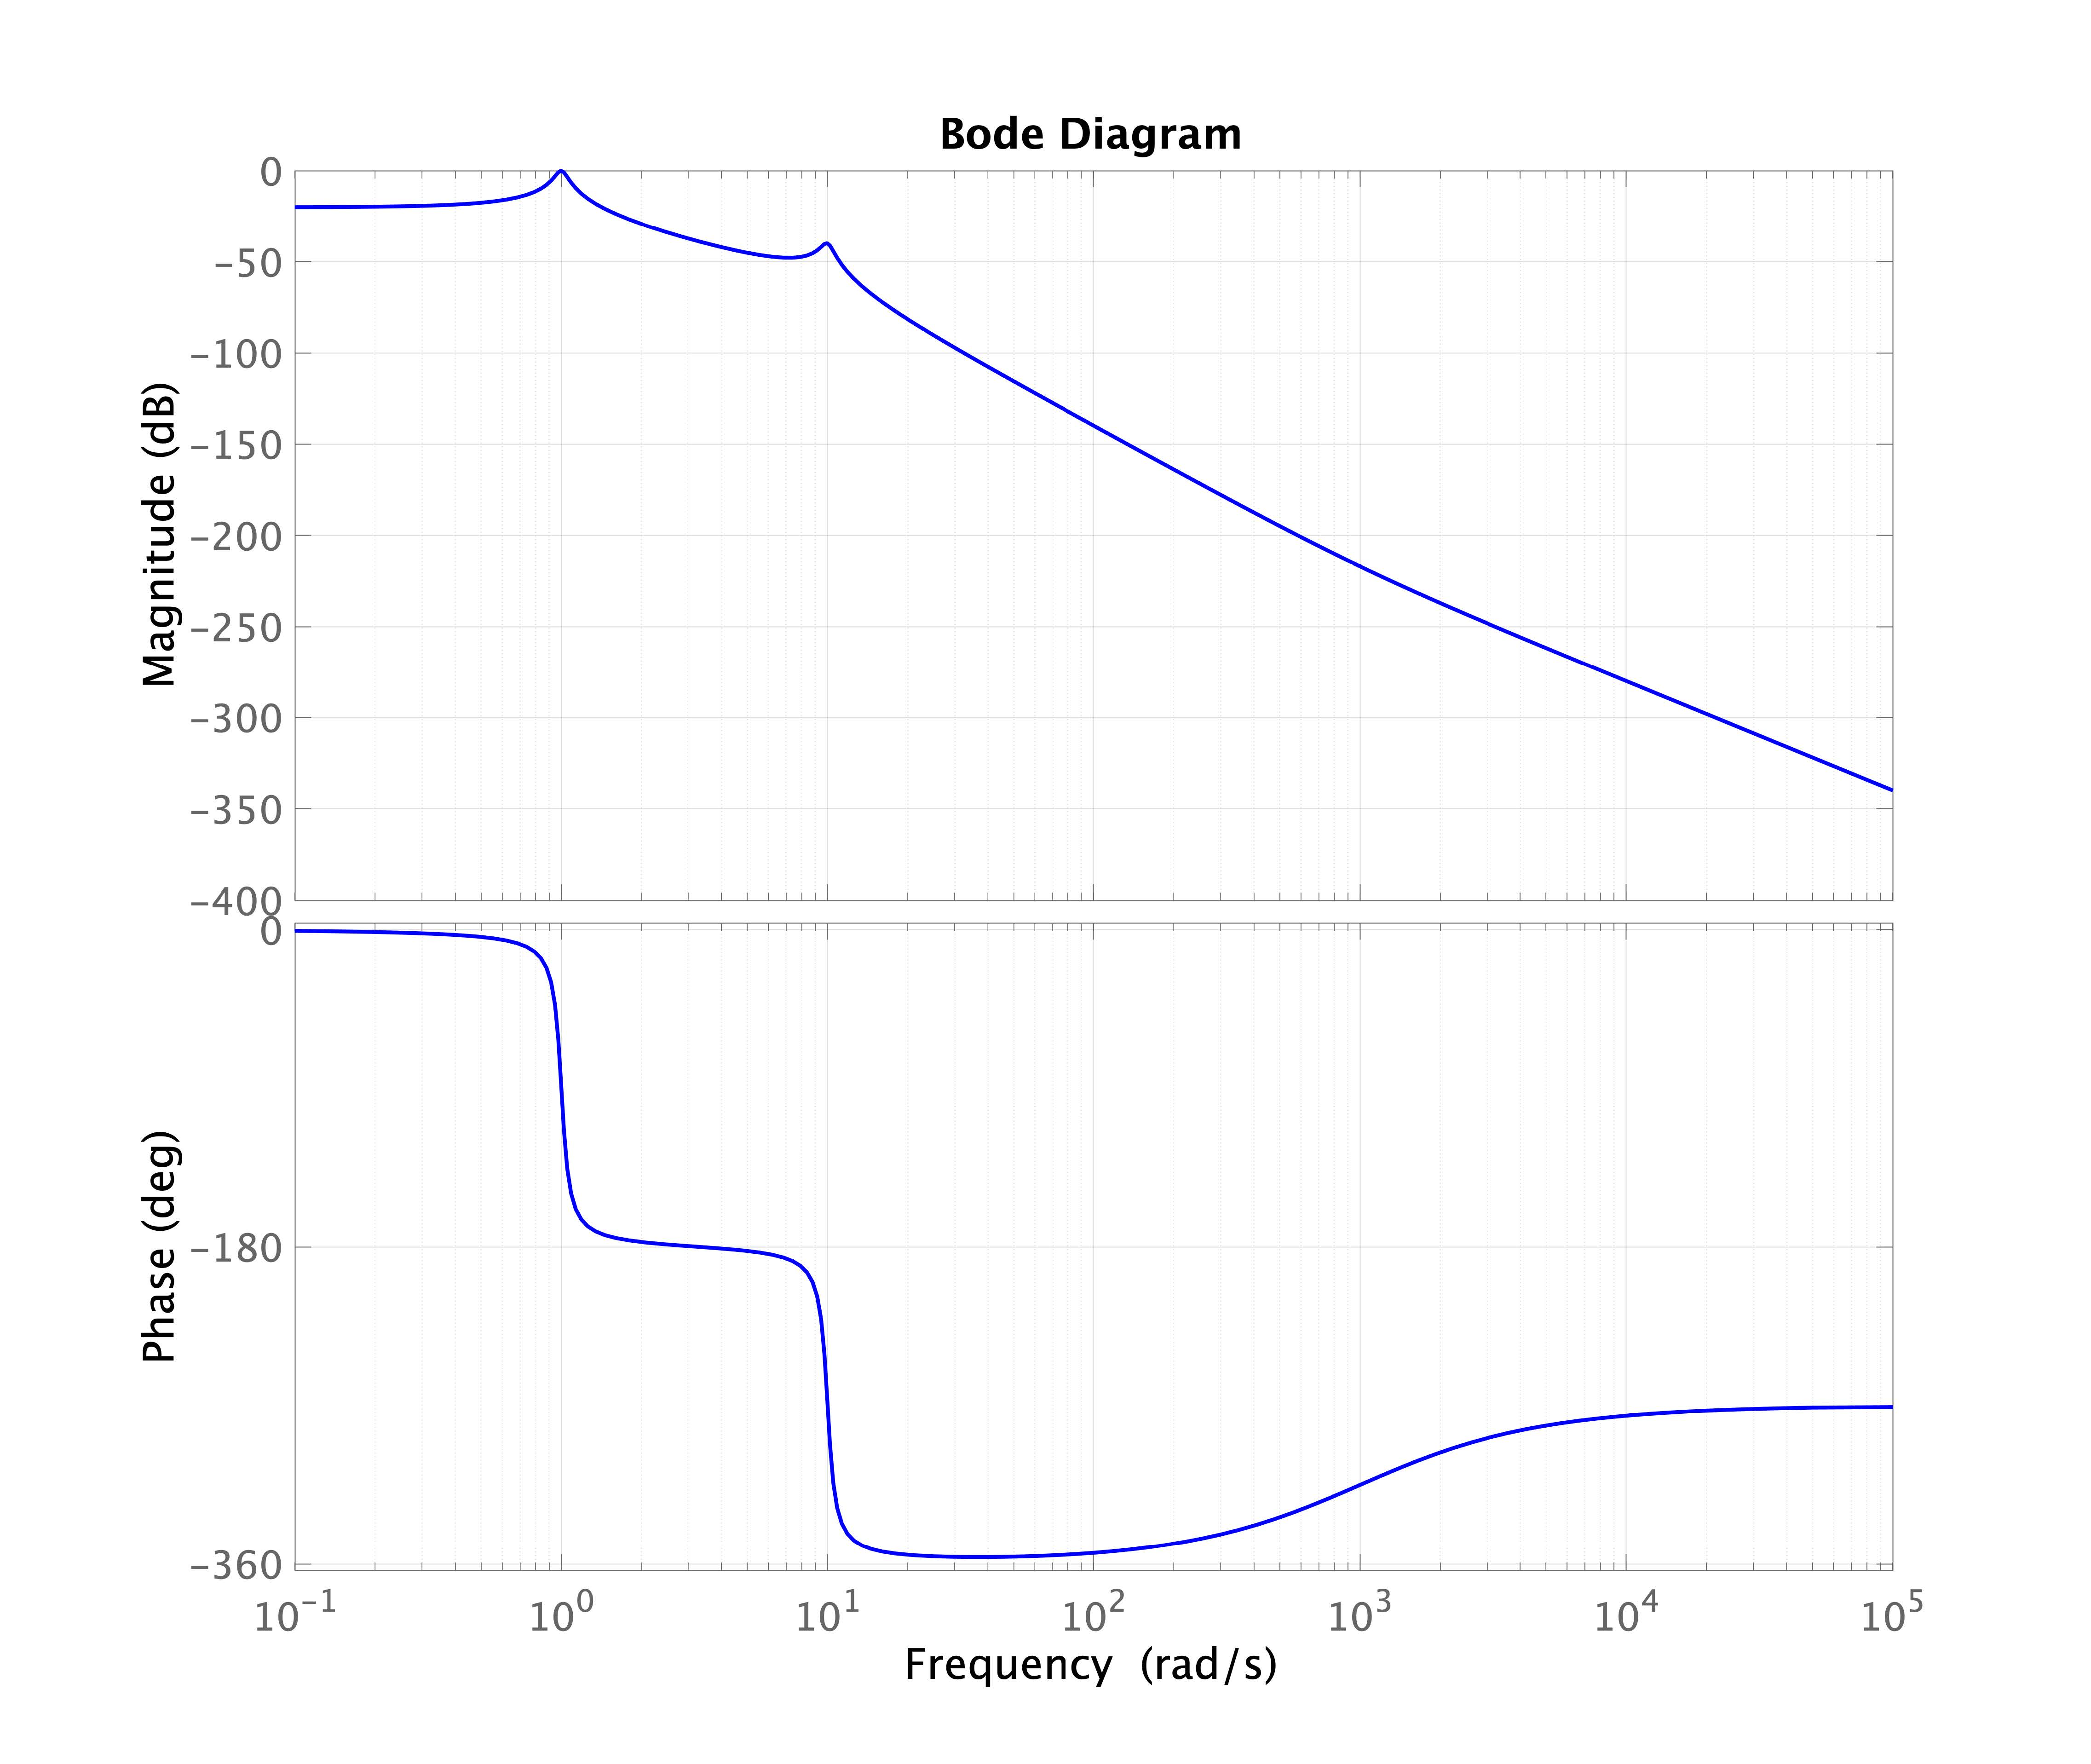
\includegraphics[width=0.5\textwidth]{figs/pblm3b.jpg}
	\caption{Bode Plot 2}
\end{figure}

\subsubsection{Gain, Poles, and Zeros:}
\begin{enumerate}
	\item \textbf{Gain:}  $-20$ db = $\frac{1}{10}$
	\item \textbf{Poles:}
	\begin{enumerate}
		\item $10^{0} = 1$ rad/s (complex)
		\item $10^{1} = 10$ rad/s (complex)
	\end{enumerate}
	\item Zeros:
	\begin{enumerate}
		\item $10^{3} = 1,000$ rad/s
	\end{enumerate}
\end{enumerate}

\subsubsection{Transfer Function:}\[
	H(s) = \cfrac{
			(1 + \frac{s}{1000})
		}{
			10 \qty(
				\frac{1}{1}\qty(s^2 + 2(\frac{1}{10})(1)s + (1)^2)
			) \qty(
				\frac{1}{10}\qty(s^2 + 2(\frac{1}{10})(10)s + (10)^2)
			)
		} = \cfrac{
			(s+1000)
		}{
			\qty(s^2 + 0.2 s + 1) \qty(s^2 + 2s + 100)
		}
\]
Assuming a Q-factor of around 10 to get the complex response.


\subsubsection{Cross-over Frequency:}
\begin{enumerate}
	\item $\omega_c = 10^{0} = 1$ rad/s
	\item $\omega_{180} = 10^{3} = 100$ rad/s
\end{enumerate}



\newpage
\section{Problem 4}
Consider the interconection of Problem 1 with the PI controller\[
	C(s) = \cfrac{10 (s+3)}{s}
\] and plant \[
	P(s) = \cfrac{-0.5(s^2 - 2000)}{(s-3)(s^2 + 50s + 1000)}
\]

\subsection{Is the feedback system stable? Why?}
\begin{align*}
	\cfrac{C(s) P(s)} {1 + C(s) P(s)}
		&= \cfrac{
			\cfrac{10 (s+3)}{s} \cfrac{-0.5(s^2 - 2000)}{(s-3)(s^2 + 50s + 1000)}
		}{
			1 + \cfrac{10 (s+3)}{s} \cfrac{-0.5(s^2 - 2000)}{(s-3)(s^2 + 50s + 1000)}
		}\\
		&\approx \cfrac{
			-5 s (s+3) (s-3) (s^2 - 2000) (s^2 + 50s + 1000)
		}{
			s (s-3) (s^2 + 11.73s + 73.9) (s^2 + 30.27s + 406) (s^2 + 50s + 1000)
		}
\end{align*}
Yes and No. 
Internally it is not fully stable since it has a pole/zero pair at $s=3$;
however, if we only care about TF after cancellations, then it is stable.

\subsection{Find phase and cross-over frequencies.}

\textbf{Problem:}
Use the Bode plot of the open loop transfer function $L(s) = C(s)P(s)$ to find the phase cross-over frequencies $\omega_0$ such that $L(j\omega_0) = 180\deg$. 
Use this information to compute the gain margin(s) of the feedback system. 
Check your answers using the \emph{allmargin} command in MATLAB.

\begin{figure}[h]\label{fig:pblm4b}
	\centering
	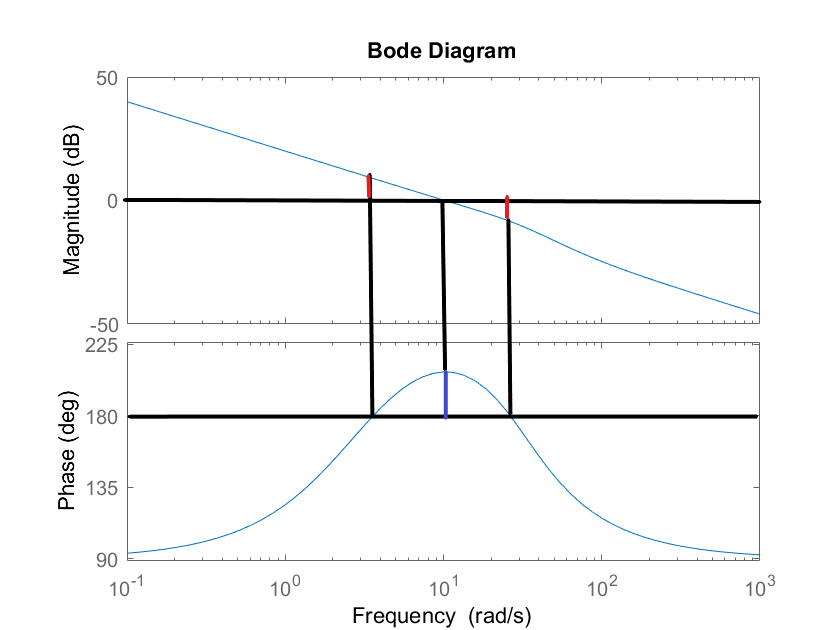
\includegraphics[width=0.7\textwidth]{figs/pblm4_L_bode.png}
	\caption{Open Loop Bode Plot of $L(S) = C(s) P(s)$}
\end{figure}

\textbf{Solution:}
As marked in the Bode Plot seen in \figurename \ \ref{fig:pblm4b}, 
the gain cross-over frequency is $\omega_{c} = 10$ resulting in a phase margin around $25\deg$.
Similarly, the phase cross-over occurs around $\omega_{180} = 4$ or $\omega_{180} = 25$, resulting in gain margins of around $\pm 10$ dB or around $g_0 = 0.3$ and $g_0 = 3$ respectively.

Verification with \emph{allmargin} resulted in similar and likely more precise and accurate results:
\begin{enumerate}
	\item Gain Margin(s)
	\begin{enumerate}
		\item $g_0 = 0.3585$ at $\omega_{180} =  3.5966$
		\item $g_0 = 2.6490$ at $\omega_{180} = 26.3797$
	\end{enumerate}
	\item Phase Margin
	\begin{enumerate}
		\item $PM = 27.5718$ at $\omega_{c} = 10.2049$
	\end{enumerate}
\end{enumerate}

\subsection{Gain Margin Closed-loop poles}
\textbf{Problem:} 
For each gain margin $g_0$ obtained in the previous part, construct the closed-loop using the perturbed loop transfer function $g_0 L(s)$ and verify that the closed-loop has poles at $\pm \omega_0$.

\textbf{Solution:}
\subsubsection{$g_0 = 0.3585$}
Let $g_0 = 0.3585$, \[
	g_0 L(s) =  \cfrac{
		-1.7927 (s+3) (s+44.72) (s-44.72)
	}{
	   s (s-3) (s^2 + 50s + 1000)
	}
\] and the closed-loop becomes \[
	H = \cfrac{ 
          -1.7927 (s-44.72) (s+44.72) (s+3)
	}{
		(s^2 + 0.0008164s + 12.93) (s^2 + 45.21s + 831.7)
	}
\] This has complex poles located at $-0.0004 \pm j 3.596$, which is essentially roots at $\pm j \omega_{180}$.


\subsubsection{$g_0 = 2.6490$}
Let $g_0 = 2.6490$, \[
	g_0 L(s) =  \cfrac{
		-13.245 (s+3) (s+44.72) (s-44.72)
	}{
	   s (s-3) (s^2 + 50s + 1000)
	}
\] and the closed-loop becomes \[
	H = \cfrac{ 
		-13.245 (s+3) (s+44.72) (s-44.72)
	}{
		(s+29.94) (s+3.814) (s^2 + 0.003402s + 696)
	}
\] This has complex poles located at $-0.0017 \pm j 26.3818$, which is essentially roots at $\pm j \omega_{180}$.

\subsection{$\norm{S-T}_\infty$}
\textbf{Problem:}
Compute $\norm{S-T}_\infty$ and the corresponding frequency $\omega_{p}$ where the peak gain of $S-T$ is achieved.

\textbf{Solution:} 








% \newpage
% \appendix
% \section{MATLAB Code:}\label{apx:matlab}
% All code I write in this course can be found on my GitHub repository:\\
% \href{https://github.com/jonaswagner2826/MECH6313}{https://github.com/jonaswagner2826/MECH6313}


\end{document}
